% !TeX spellcheck = en_US
% !TeX program = lualatex


% Do not surround the equal signs with spaces, it causes errors!
\documentclass[
	aspectratio=43,
	color={accentcolor=1c},
	logo=false,
	colorframetitle=true,
	handout
]{tudabeamer}

% Include preamble to not clutter this file.
% Core packages.
% Primary: English, Secondary: German.
\usepackage[main = english, ngerman]{babel}
% Other packages.
%\usepackage{graphicx}
\usepackage{tikz}
\usepackage{mathtools}
\usepackage{amssymb}
\usepackage{siunitx}
\usepackage{tabularx}
\usepackage{xcolor}
\usepackage[font = normalsize, labelfont = bf]{caption}
\usepackage{subcaption}
\usepackage{float}
\usepackage{wrapfig}
\usepackage[ruled, vlined, linesnumbered]{algorithm2e}
\usepackage{csquotes}
\usepackage{microtype}
\usepackage{physics}
\usepackage{cancel}
\usepackage{hyperref}
\usepackage{tabto}
\usepackage{eqparbox}
\usepackage{pgfplots}
\usepackage{multicol}
\usepackage{listings}
\usepackage{xspace}
\usepackage[bottom]{footmisc}
\usepackage{excludeonly}

\usetikzlibrary{arrows.meta, shapes, backgrounds, angles, calc, chains, scopes, decorations.pathmorphing, patterns, positioning, quotes}

% Debug packages.
\usepackage{comment}

\makeatletter

% Make LOA a section.
\newcommand{\listalgorithmname}{List of Algorithms}
\renewcommand\listofalgorithms{
	\section*{\listalgorithmname}
	\@mkboth{\MakeUppercase\listalgorithmname}{\MakeUppercase\listalgorithmname}
	\@starttoc{loa}
}
% Make LOF a section.
\renewcommand\listoffigures{
	\section*{\listfigurename}
	\@mkboth{\MakeUppercase\listfigurename}{\MakeUppercase\listfigurename}
	\@starttoc{lof}
}
% Make LOL a section.
\newcommand{\listlistingname}{List of Listings}
\newcommand\listoflistings{
	\section*{\listlistingname}
	\@mkboth{\MakeUppercase\listfigurename}{\MakeUppercase\listfigurename}
	\@starttoc{lol}
}
% Make LOT a section.
\renewcommand\listoftables{
	\section*{\listtablename}
	\@mkboth{\MakeUppercase\listtablename}{\MakeUppercase\listtablename}
	\@starttoc{lot}
}

\makeatother



% Style definitions.

% Description-list styling.
\SetLabelAlign{parright}{\parbox[t]{\labelwidth}{\raggedleft#1}}
\setlist[description]{style = multiline, leftmargin = 4cm, align = parright}

\MakeOuterQuote{"}

% Simplify command to center a caption.
\newcommand{\captioncenter}{\captionsetup{justification=centering}}

% Matrix/Vector notation.
\renewcommand{\vec}[1]{\boldsymbol{\mathrm{#1}}}
\newcommand{\mat}[1]{\boldsymbol{\mathrm{#1}}}
% Shorthands.
\renewcommand{\C}{\mathbb{C}}
\newcommand{\R}{\mathbb{R}}
\newcommand{\E}{\mathbb{E}}
\newcommand{\normal}{\mathcal{N}}
\newcommand{\gaussianMulti}[4]{\frac{1}{\left(2\pi\right)^{#4/2} \cdot \lvert #3 \rvert^{1/2}} \exp \bigg\{\! -\frac{1}{2} \left(#1 - #2\right)^T #3^{-1} \left(#1 - #2\right) \bigg\}}
\newcommand{\logGaussianMulti}[4]{-\frac{1}{2} \log \lvert #3 \rvert - \frac{#4}{2} \log\left(2\pi\right) - \frac{1}{2} \left(#1 - #2\right)^T #3^{-1} \left(#1 - #2\right)}
\newcommand{\subgiven}{\vert}
\newcommand{\given}{\,\vert\,}
\newcommand{\biggiven}{\,\big\vert\,}
\newcommand{\Biggiven}{\,\Big\vert\,}
\newcommand{\bigggiven}{\,\bigg\vert\,}
\newcommand{\Bigggiven}{\,\Bigg\vert\,}
\newcommand{\new}{\mathrm{new}}
\newcommand{\KL}[2]{D_\mathrm{KL}\big( #1 \,\Vert\, #2 \big)}
\newcommand{\SRC}{\mathit{SRC}}
\newcommand{\rangedots}{\,\cdots\!}
\newcommand{\train}{\mathrm{train}}
% Math operators.
\DeclareMathOperator{\const}{const}
\DeclareMathOperator{\Cov}{Cov}
\DeclareMathOperator{\diag}{diag}

\newcommand{\oversetfootnotemark}[1]{\stepcounter{footnote} \overset{\mathclap{(\thefootnote)}}{#1}}
\let\realfootnote\footnote
\let\realfootnotetext\footnotetext
\renewcommand{\footnote}[1]{\realfootnote{\, #1}}
\renewcommand{\footnotetext}[1]{\realfootnotetext{\, #1}}
\newcommand{\doublefootnotetext}[2]{\addtocounter{footnote}{-1} \footnotetext{#1} \stepcounter{footnote} \footnotetext{#2}}
\newcommand{\triplefootnotetext}[3]{\addtocounter{footnote}{-2} \footnotetext{#1} \stepcounter{footnote} \footnotetext{#2} \stepcounter{footnote} \footnotetext{#3}}

\parindent0pt

% Definitions, Theorems and Lemmata.
\newtheorem{theorem}{Theorem}[chapter]
\newtheorem{definition}[theorem]{Definition}
\newtheorem{lemma}[theorem]{Lemma}

% Do not include subsections and lower in TOC.
\setcounter{tocdepth}{1}

% BibTeX.
\renewcommand{\bibname}{References}
%\bibliographystyle{ieeetr}
\bibliographystyle{alpha}

% TikZ-related stuff.
\tikzset{> = { Latex[length = 2mm] }}

% algorithm2e.
\SetCommentSty{text}

% Listings.
\colorlet{changedpurple}{TUDa-11a}
\colorlet{lerrorred}{TUDa-9b}
\colorlet{lstcomments}{TUDa-4c}
\colorlet{lstkeywords}{TUDa-9d}
\colorlet{lstlinenumbers}{TUDa-0c}
\colorlet{lststrings}{TUDa-2c}
\lstdefinestyle{base}{
	moredelim = **[is][\color{errorred}]{@@!}{@@@},
	moredelim = **[is][\color{changedpurple}]{@@?}{@@@}
}
\lstset{
	backgroundcolor   = \color{white},
	basicstyle        = \ttfamily\scriptsize\color{black},
	breakatwhitespace = true,
	breaklines        = true,
	breakautoindent   = true,
	captionpos        = b,
	commentstyle      = \color{lstcomments},
	escapeinside      = {{*@}{@*}},
	keywordstyle      = \color{lstkeywords},
	language          = Python,
	numbers           = left,
	numberstyle       = \tiny\color{lstlinenumbers},
	showstringspaces  = false,
	stringstyle       = \color{lststrings},
	style             = base,
	tabsize           = 4
}

% Ignore well-known acronyms in write-first-long rule.
% TODO: Replace the usage of \ac{..} with these everywhere!
\newcommand{\eg}{\acrshort{eg}\xspace}
\newcommand{\ie}{\acrshort{ie}\xspace}
\newcommand{\wrt}{\acrshort{wrt}\xspace}

% Other.
\newcommand{\appautorefname}{appendix}



% Glossary styles.
\newcolumntype{L}[1]{>{\raggedright\let\newline\\\arraybackslash\hspace{0pt}}m{#1}}
\newcolumntype{C}[1]{>{\centering\let\newline\\\arraybackslash\hspace{0pt}}m{#1}}
\newcolumntype{R}[1]{>{\raggedleft\let\newline\\\arraybackslash\hspace{0pt}}m{#1}}
\newglossarystyle{iasThesisGeneral}{
	\glossarystyle{super3colheader}%
	\renewenvironment{theglossary}%
		{\begin{longtable}{L{0.15\textwidth}L{0.8\textwidth}R{0\textwidth}}}%
		{\end{longtable}}%
	\renewcommand*{\glossaryheader}{\textbf{\entryname} & \textbf{\descriptionname} & \\}
	\renewcommand*{\glossaryentryfield}[5]{\glsentryitem{##1}\glstarget{##1}{##2} & ##3 \\}
}
\newglossarystyle{iasThesisOperators}{
	\glossarystyle{super3colheader}
	\renewenvironment{theglossary}
		{\begin{longtable}{L{0.15\textwidth}L{0.55\textwidth}L{0.25\textwidth}}}%
		{\end{longtable}}%
	\renewcommand*{\glossaryheader}{\textbf{\entryname} & \textbf{\descriptionname} & \textbf{Operator} \\}
	\renewcommand*{\glossaryentryfield}[5]{\glsentryitem{##1}\glstarget{##1}{##2} & ##3 & ##4 \\}
}

% Tikz-diagrams for not cluttering the text.

\newcommand{\tikzHarmonicOscillator}{
	\begin{tikzpicture}
		\node [draw, rectangle] (m) at (0, 3) {\(m\)};
		\draw [thick] (-1.5, 5) -- (1.5, 5);
		\fill [pattern = north east lines] (-1.5, 5) rectangle (1.5, 5.2);
		\draw [decoration = { aspect = 0.3, segment length = 2mm, amplitude = 3mm, coil }, decorate] (0, 5) -- node[left, xshift = -0.4cm]{\(k\)} (m);

		\coordinate (xA) at (1, 4.5);
		\coordinate (xB) at (1, 3.5);
		\draw [->] (xA) -- node[right]{\(x\)} (xB);
	\end{tikzpicture}
}

\newcommand{\tikzSimplePendulum}{
	\begin{tikzpicture}
		\node [draw, circle, fill, minimum width = 0.5cm] (C) at (0, 0) {};
		\node [draw, circle] (mass) at (120:3cm) {\(m\)};
		\coordinate (A) at (90:3cm);
		\draw (C) -- node[left]{\(L\)} (mass);
		\draw [dashed] (C) -- (A);
		\draw pic [draw, "$\varphi$", angle radius = 1.5cm] {angle=A--C--mass};

		\draw [<-] (0.5, 1) -- node[right]{\(g\)} (0.5, 2);
	\end{tikzpicture}
}

\newcommand{\tikzKoopmanOperator}{
	\begin{tikzpicture}[->, state/.style = { draw, circle, minimum width = 1cm, minimum height = 1cm }]
		\node [state]                  (y1) {\raisebox{-5pt}{\(\vec{y}_{\,\mathclap{\,1}}\)}};
		\node [state, right = 1 of y1] (y2) {\raisebox{-5pt}{\(\vec{y}_{\,\mathclap{\,2}}\)}};
		\node [state, right = 1 of y2] (y3) {\raisebox{-5pt}{\(\vec{y}_{\,\mathclap{\,3}}\)}};
		\node [minimum width = 1cm, minimum height = 1cm, right = 1 of y3] (yD) {\(\cdots\)};
		\node [state, right = 1 of yD] (yT) {\raisebox{-5pt}{\(\vec{y}_{\,\mathclap{\,T}}\)}};

		\node [state, below = 1 of y1] (x1) {\raisebox{-5pt}{\(\vec{x}_{\,\mathclap{\,1}}\)}};
		\node [state, below = 1 of y2] (x2) {\raisebox{-5pt}{\(\vec{x}_{\,\mathclap{\,2}}\)}};
		\node [state, below = 1 of y3] (x3) {\raisebox{-5pt}{\(\vec{x}_{\,\mathclap{\,3}}\)}};
		\node [minimum width = 1cm, minimum height = 1cm, below = 1 of yD] (xD) {\(\cdots\)};
		\node [state, below = 1 of yT] (xT) {\raisebox{-5pt}{\(\vec{x}_{\,\mathclap{\,T}}\)}};

		\draw (y1) -- node[above]{\(\mathcal{K}\)} (y2);
		\draw (y2) -- node[above]{\(\mathcal{K}\)} (y3);
		\draw (y3) -- node[above]{\(\mathcal{K}\)} (yD);
		\draw (yD) -- node[above]{\(\mathcal{K}\)} (yT);

		\draw (x1) -- node[below]{\(\vec{F}\)} (x2);
		\draw (x2) -- node[below]{\(\vec{F}\)} (x3);
		\draw (x3) -- node[below]{\(\vec{F}\)} (xD);
		\draw (xD) -- node[below]{\(\vec{F}\)} (xT);

		\draw (y1) to[bend right = 15] node[left]{\(\vec{g}\)} (x1);
		\draw (y2) to[bend right = 15] node[left]{\(\vec{g}\)} (x2);
		\draw (y3) to[bend right = 15] node[left]{\(\vec{g}\)} (x3);
		\draw (yT) to[bend right = 15] node[left]{\(\vec{g}\)} (xT);

		\draw [dashed] (x1) to[bend right = 15] node[right]{\(\vec{g}^{-1}\)} (y1);
		\draw [dashed] (x2) to[bend right = 15] node[right]{\(\vec{g}^{-1}\)} (y2);
		\draw [dashed] (x3) to[bend right = 15] node[right]{\(\vec{g}^{-1}\)} (y3);
		\draw [dashed] (xT) to[bend right = 15] node[right]{\(\vec{g}^{-1}\)} (yT);
	\end{tikzpicture}
}

\newcommand{\tikzHiddenMarkovModel}{
	\begin{tikzpicture}[->, state/.style = { draw, circle, minimum width = 1cm, minimum height = 1cm }]
		\node [state]                  (s1) {\raisebox{-5pt}{\(s_{\,\mathclap{\,1}}\)}};
		\node [state, right = 1 of s1] (s2) {\raisebox{-5pt}{\(s_{\,\mathclap{\,2}}\)}};
		\node [state, right = 1 of s2] (s3) {\raisebox{-5pt}{\(s_{\,\mathclap{\,3}}\)}};
		\node [minimum width = 1cm, minimum height = 1cm, right = 1 of s3] (sD) {\(\cdots\)};
		\node [state, right = 1 of sD] (sT) {\raisebox{-5pt}{\(s_{\,\mathclap{\,T}}\)}};

		\node [state, below = 1 of s1] (y1) {\raisebox{-5pt}{\(\vec{y}_{\,\mathclap{\,1}}\)}};
		\node [state, below = 1 of s2] (y2) {\raisebox{-5pt}{\(\vec{y}_{\,\mathclap{\,2}}\)}};
		\node [state, below = 1 of s3] (y3) {\raisebox{-5pt}{\(\vec{y}_{\,\mathclap{\,3}}\)}};
		\node [state, below = 1 of sT] (yT) {\raisebox{-5pt}{\(\vec{y}_{\,\mathclap{\,T}}\)}};

		\draw (s1) -- (s2);
		\draw (s2) -- (s3);
		\draw (s3) -- (sD);
		\draw (sD) -- (sT);

		\draw (s1) -- (y1);
		\draw (s2) -- (y2);
		\draw (s3) -- (y3);
		\draw (sT) -- (yT);
	\end{tikzpicture}
}

\newcommand{\tikzLinearGaussianDynamicalSystem}{
	\begin{tikzpicture}[->, state/.style = { draw, circle, minimum width = 1cm, minimum height = 1cm }]
		\node [state]                  (x1) {\raisebox{-5pt}{\(\vec{x}_{\,\mathclap{\,1}}\)}};
		\node [state, right = 1 of x1] (x2) {\raisebox{-5pt}{\(\vec{x}_{\,\mathclap{\,2}}\)}};
		\node [state, right = 1 of x2] (x3) {\raisebox{-5pt}{\(\vec{x}_{\,\mathclap{\,3}}\)}};
		\node [minimum width = 1cm, minimum height = 1cm, right = 1 of x3] (xD) {\(\cdots\)};
		\node [state, right = 1 of xD] (xT) {\raisebox{-5pt}{\(\vec{x}_{\,\mathclap{\,T}}\)}};

		\node [state, below = 1 of x1] (y1) {\raisebox{-5pt}{\(\vec{y}_{\,\mathclap{\,1}}\)}};
		\node [state, below = 1 of x2] (y2) {\raisebox{-5pt}{\(\vec{y}_{\,\mathclap{\,2}}\)}};
		\node [state, below = 1 of x3] (y3) {\raisebox{-5pt}{\(\vec{y}_{\,\mathclap{\,3}}\)}};
		\node [state, below = 1 of xT] (yT) {\raisebox{-5pt}{\(\vec{y}_{\,\mathclap{\,T}}\)}};

		\draw (x1) -- node[above]{\(\mat{A}\)} (x2);
		\draw (x2) -- node[above]{\(\mat{A}\)} (x3);
		\draw (x3) -- node[above]{\(\mat{A}\)} (xD);
		\draw (xD) -- node[above]{\(\mat{A}\)} (xT);

		\draw (x1) -- node[left]{\(\mat{C}\)} (y1);
		\draw (x2) -- node[left]{\(\mat{C}\)} (y2);
		\draw (x3) -- node[left]{\(\mat{C}\)} (y3);
		\draw (xT) -- node[left]{\(\mat{C}\)} (yT);
	\end{tikzpicture}
}



\title{Variational Autoencoders for Koopman Dynamical Systems}
\subtitle{B.Sc. Thesis Defense}
\author{Fabian Damken}
\department{Department of Computer Science}
\institute{Intelligent Autonomous Systems}
\date{December 10, 2020}

\logo*{\includegraphics{img/iasLogo}}

\titlegraphic*{\includegraphics{figures/title}}

\newcommand{\hence}{\(\longrightarrow\,\)}

\begin{document}
	\maketitle

	\section{Introduction}
		\begin{frame}{Motivation}
			\begin{itemize}
				\item Control theory for linear systems is highly evolved.
				\item But nonlinear systems are hard\dots
				\item We need ways to linearize a nonlinear system!
				\item<2-> "Classical" Linearization:
					\begin{itemize}
						\item Use small angle approximation (e.g. for pendulum)?
						\item Diverge fast with higher displacements\dots
						\item Only linearize locally, not globally.
					\end{itemize}
				\item<3-> Koopman theory offers a way to do that!
			\end{itemize}
		\end{frame}

		\begin{frame}{The Koopman Operator}
			For a \emph{nonlinear} dynamical system
			\begin{align*}
				\vec{x}_{t + 1} = \vec{F}(\vec{x}_{t})
			\end{align*}
			with \emph{nonlinear} measurements (an \emph{embedding})
			\begin{align*}
				\vec{y}_t = \vec{h}(\vec{x}_t)
			\end{align*}
			the Koopman operator advances these measurements forward in time \emph{linearly}:
			\begin{align*}
				\vec{h}(\vec{x}_{t + 1}) = \mathcal{K} \vec{h}(\vec{x}_t)
				\quad\iff\quad
				\vec{y}_{t + 1} = \mathcal{K} \vec{x}_t
			\end{align*}

			This is possible for every nonlinear dynamical system. And globalizes linearly! But the embedding \(\vec{h}\) is typically infinite-dimensional\dots
		\end{frame}

		\begin{frame}[c]{Koopman Dynamical System}
			\begin{center}
				\tikzKoopmanOperator
			\end{center}
			\begin{center}
				\small
				Adopted from Brunton et al. "Koopman Invariant Subspaces and Finite Linear Representations of Nonlinear Dynamical Systems for Control".
			\end{center}
		\end{frame}

		\begin{frame}[c]{Linear Gaussian Dynamical System}
			\begin{center}
				\tikzLinearGaussianDynamicalSystem
			\end{center}

			\begin{equation*}
				\begin{aligned}
					\vec{s}_{t + 1} &= \eqmakebox[a][l]{\( \mat{A} \vec{s}_t + \vec{w}, \)}\quad \eqmakebox[b][r]{\( \vec{w} \)} \sim \normal(\vec{0}, \mat{Q}) \\
					\vec{y}_t &= \eqmakebox[a][l]{\( \mat{C} \vec{s}_t + \vec{v}, \)}\quad \eqmakebox[b][r]{\( \vec{v} \)} \sim \normal(\vec{0}, \mat{R})
				\end{aligned}
				\qquad\iff\qquad
				\begin{aligned}
					\vec{s}_{t + 1} &\sim \normal(\mat{A} \vec{s}_t, \mat{Q}) \\
					\vec{y}_t &\sim \eqmakebox[c][l]{\(\normal(\mat{C} \vec{s}_t, \mat{R})\)}
				\end{aligned}
			\end{equation*}
		\end{frame}
	% end

	\section{Koopman Inference}
		\begin{frame}[c]{The Koopman Inference Model}
			\begin{center}
				\tikzNonlinearGaussianKoopman
			\end{center}

			\begin{equation*}
				\begin{aligned}
					\vec{s}_{t + 1} &= \eqmakebox[a][l]{\( \mat{A} \vec{s}_t + \vec{w}, \)}\quad \eqmakebox[b][r]{\( \vec{w} \)} \sim \normal(\vec{0}, \mat{Q}) \\
					\vec{y}_t &= \eqmakebox[a][l]{\( {\color{TUDa-9b} \vec{g}(\vec{s}_t)} + \vec{v}, \)}\quad \eqmakebox[b][r]{\( \vec{v} \)} \sim \normal(\vec{0}, \mat{R})
				\end{aligned}
				\qquad\iff\qquad
				\begin{aligned}
					\vec{s}_{t + 1} &\sim \normal(\mat{A} \vec{s}_t, \mat{Q}) \\
					\vec{y}_t &\sim \eqmakebox[c][l]{\(\normal({\color{TUDa-9b} \vec{g}(\vec{s}_t)}, \mat{R})\)}
				\end{aligned}
			\end{equation*}
		\end{frame}

		\begin{frame}{How to learn?}
			Goal: Estimate all of the following:
			\begin{itemize}
				\item Latent dynamics matrix \( \mat{A} \).
				\item Measurement function \( \vec{g}_{\vec{\theta}}(\cdot) \) (\ie the parameters \(\vec{\theta}\)). \\ Variational auto-encoder without an amortization network.
				\item Noise covariances \(\mat{Q}\), \(\mat{R}\).
			\end{itemize}
			We employ an EM-algorithm to do that.

			\onslide<2->{
				\begin{alertblock}{Core Problem}
					Some expectations cannot be evaluated in closed form for a nonlinear \( \vec{g}_{\vec{\theta}}(\cdot) \).
				\end{alertblock}
			}

			\onslide<3->{
				\begin{itemize}
					\item Use cubature rules for evaluating the intractable expectations.
					\item No closed form solution for maximizing w.r.t. function parameters \( \vec{\theta} \).
					\item<4->[] \(\qquad\longrightarrow\quad\) Use backpropagation and gradient descent!
				\end{itemize}
			}
		\end{frame}
	% end

	\section{Related Work}
		\begin{frame}{Related Work}
			\begin{itemize}
				\item<+-> Lusch et al. "Deep Learning for Universal Linear Embeddings of Nonlinear Dynamics":
					\begin{itemize}
						\item Use an autoencoder approach with an encoder network.
						\item No probabilistic interpretation.
				\end{itemize}
				\item<+-> Morton et al. "Deep Variational Koopman Models: Inferring Koopman Observations for Uncertainty-Aware Dynamics Modeling and Control":
					\begin{itemize}
						\item Utilize six different neural networks to perform variational inference.
						\item Very complex model, lots of parameters.
						\item Utilize much more training data than our method.
					\end{itemize}
				\item<+-> Becker et al. "Recurrent Kalman Networks: Factorized Inference in High-Dimensional Deep Feature Spaces"
					\begin{itemize}
						\item Proposal of a new type of recurrent neural networks: Kalman network.
						\item Uses high-dimensional linear embeddings with factorized covariances. \\
							\quad \(\longrightarrow\,\) Simple Kalman update rules.
					\end{itemize}
%				\item<+-> Zhang, Vikram et al. "SOLAR: Deep Structured Representations for Model-Based Reinforcement Learning"
			\end{itemize}
		\end{frame}
	% end

	\section{Experiments}
		\begin{frame}{Experimental Questions and Environments}
			\begin{enumerate}
				\item How does the latent dimensionality affect the model performance?
				\item How does our model perform in relation to the DVK model?
				\item How do different feature transformations of the environment affect the model performance?
			\end{enumerate}

			\onslide<2->{
				\vspace{0.5cm}
				Environments:
				\begin{itemize}
					\item \eqmakebox[envs][l]{Pendulum:}                         \(\theta\),\, \(\dot{\theta}\)
					\item \eqmakebox[envs][l]{\textbf<2->{Damped Pendulum:}}     \(\theta\),\, \(\dot{\theta}\)
					\item \eqmakebox[envs][l]{Gym Pendulum:}                     \(\cos\theta\),\, \(\sin\theta\),\, \(\dot{\theta}\)
					\item \eqmakebox[envs][l]{Gym Cartpole:}                     \(x\),\, \(\dot{x}\),\, \(\theta\),\, \(\dot{\theta}\)
					\item \eqmakebox[envs][l]{\textbf<2->{Gym Double Pendulum:}} \(\cos\varphi_1\),\, \(\sin\varphi_1\),\, \(\cos\varphi_2\),\, \(\sin\varphi_2\),\, \(\dot{\varphi}_1\),\, \(\dot{\varphi}_2\)
				\end{itemize}
			}
		\end{frame}

		\subsection{Damped Pendulum}
			\begin{frame}{Damped Pendulum}
				\vspace{-0.5cm}
				\begin{equation*}
					m\ddot{\theta} = \frac{g}{L} \sin\theta - d \dot{\theta}
					\quad\longrightarrow\quad
					\ddot{\theta} = \sin\theta - 0.1 \dot{\theta}
				\end{equation*}

				\begin{columns}[c]
					\begin{column}{0.35\linewidth}
						Observations:
						\begin{itemize}
							\item \eqmakebox[pendulum][l]{Displacement:} \(\theta\)
							\item \eqmakebox[pendulum][l]{Velocity:}     \(\dot{\theta}\)
						\end{itemize}
						\begin{center}
							\resizebox{0.85\linewidth}{!}{\tikzSimplePendulum}
						\end{center}
					\end{column}
					\begin{column}{0.65\linewidth}
						\begin{center}
							\includegraphics<2->[width=\linewidth]{figures/experiments/pendulum-damped/log-likelihood.pdf}
						\end{center}
					\end{column}
				\end{columns}
			\end{frame}

			\begin{frame}[c]{Rollout in Observation Space}{Damped Pendulum}
				\begin{center}
					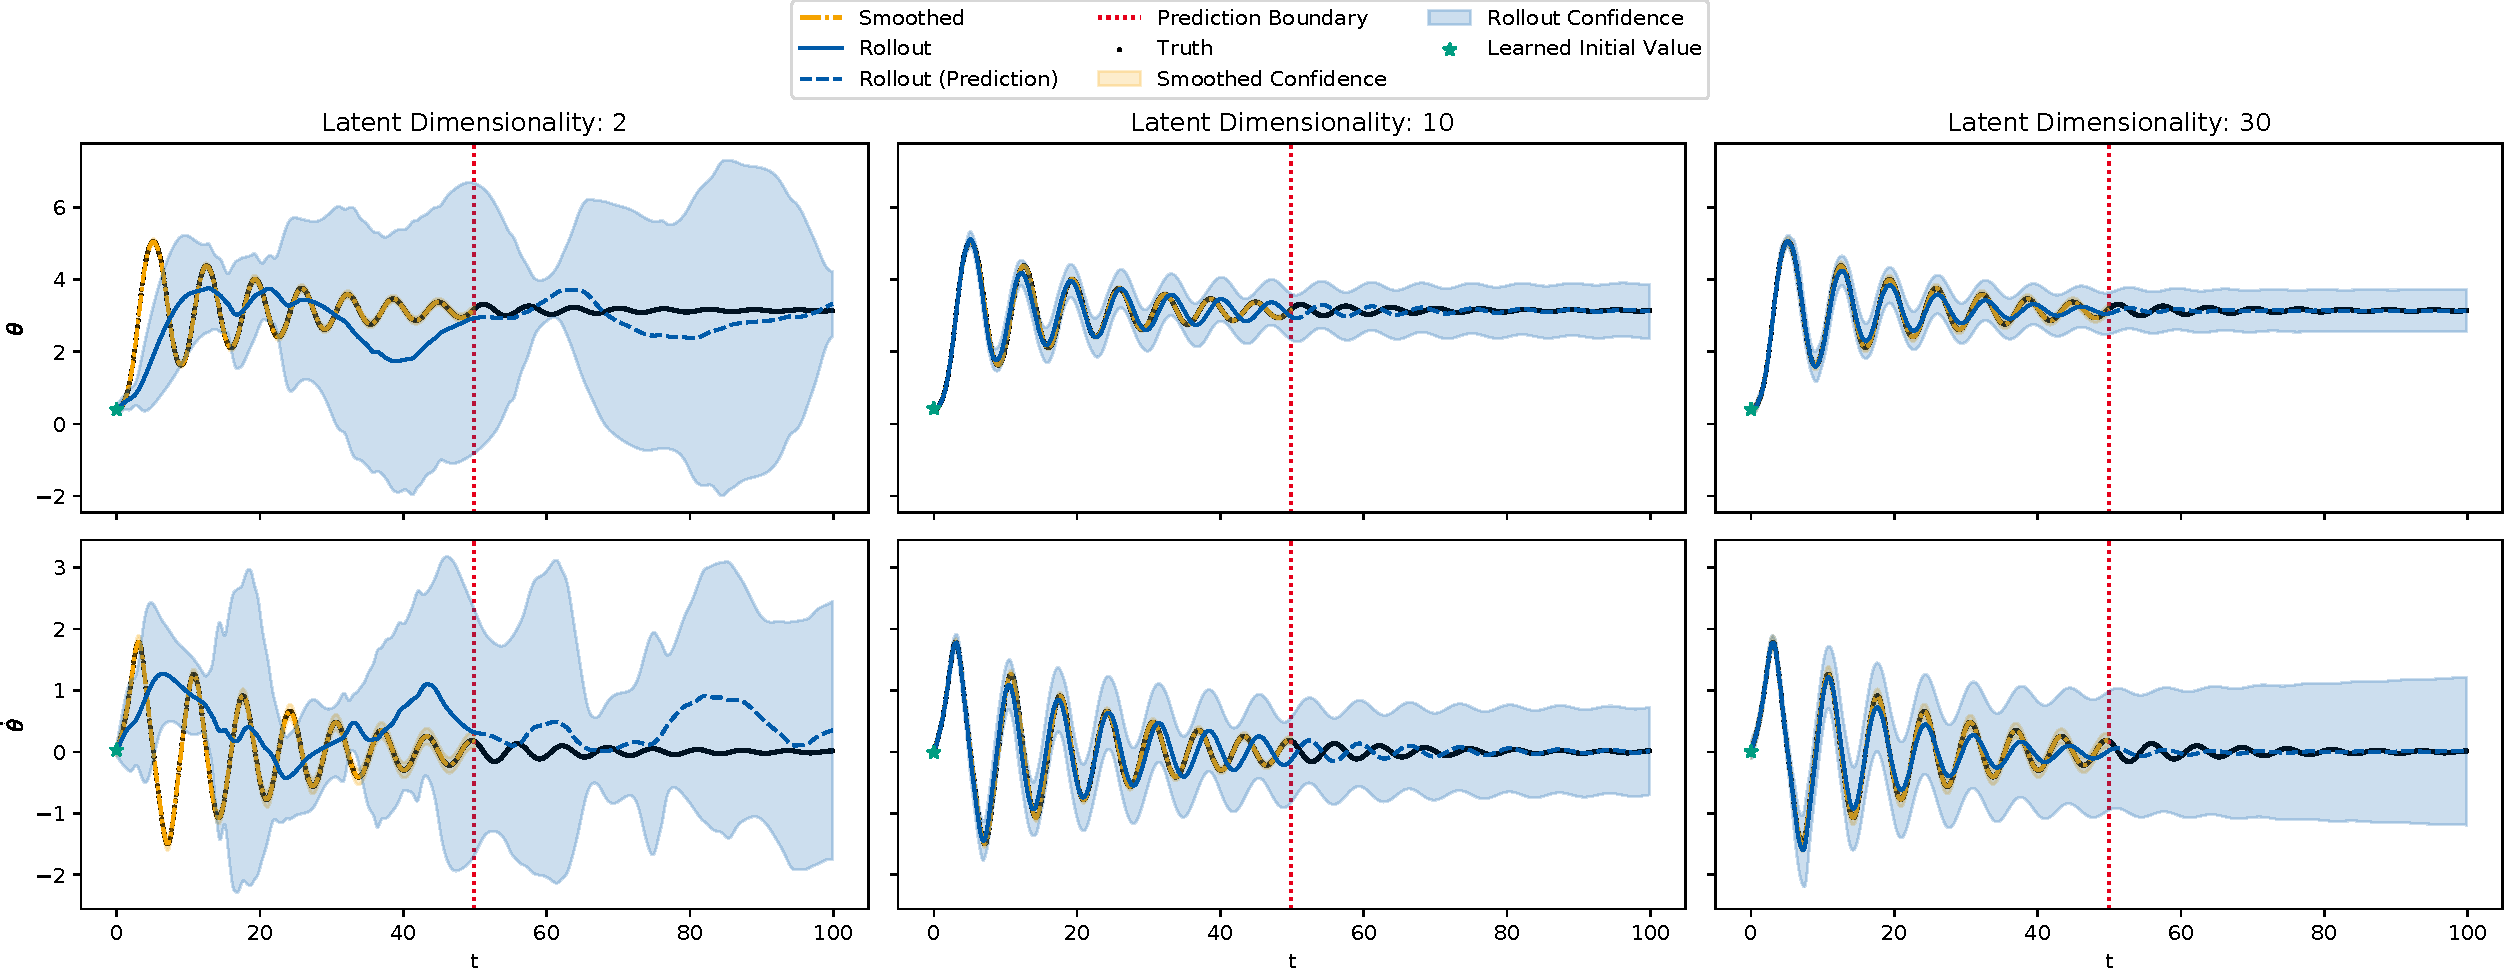
\includegraphics[width=\linewidth]{figures/experiments/pendulum-damped/different-latent-dims-rollouts.pdf}
				\end{center}
			\end{frame}

			\begin{frame}[c]{Effect of the Latent Dimensionality}{Damped Pendulum}
				\begin{columns}[c]
					\begin{column}{0.5\linewidth}
						\begin{center}
							\includegraphics[width=\linewidth]{figures/experiments/pendulum-damped/latent-dim/comparison-rmse-rollout-train-mean-vs-latent-dim.pdf}
						\end{center}
					\end{column}
					\begin{column}{0.5\linewidth}
						\begin{center}
							\includegraphics[width=\linewidth]{figures/experiments/pendulum-damped/latent-dim/comparison-rmse-rollout-prediction-mean-vs-latent-dim.pdf}
						\end{center}
					\end{column}
				\end{columns}
			\end{frame}

			\begin{frame}[c]{Exemplary Run and Energy, 10 Latents}{Damped Pendulum}
				\begin{center}
					\includegraphics[width=\linewidth]{figures/experiments/pendulum-damped/rollout-observations-N0.pdf}
				\end{center}
				\vspace{-1cm}
				\begin{columns}
					\begin{column}{0.333\linewidth}
						\begin{center}
							\includegraphics[width=\linewidth]{figures/experiments/pendulum-damped/energy-R110-N0-total.pdf}
						\end{center}
					\end{column}
					\begin{column}{0.333\linewidth}
						\begin{center}
							\includegraphics[width=\linewidth]{figures/experiments/pendulum-damped/energy-R110-N0-kinetic.pdf}
						\end{center}
					\end{column}
					\begin{column}{0.333\linewidth}
						\begin{center}
							\includegraphics[width=\linewidth]{figures/experiments/pendulum-damped/energy-R110-N0-potential.pdf}
						\end{center}
					\end{column}
				\end{columns}
			\end{frame}
		% end

		\subsection{Double Pendulum}
			\begin{frame}{Double Pendulum}
				\begin{columns}[c]
					\begin{column}{0.35\linewidth}
						Observations:
						\begin{itemize}
							\item \eqmakebox[doublePendulum][l]{Displacements:} \\
								\quad \(\cos\varphi_1\),\, \(\sin\varphi_1\), \\
								\quad \(\cos\varphi_2\),\, \(\sin\varphi_2\)
							\item Velocities: \(\dot{\varphi}_1\),\, \(\dot{\varphi}_2\)
						\end{itemize}
						\begin{center}
							\resizebox{0.85\linewidth}{!}{\tikzDoublePendulum}
						\end{center}
					\end{column}
					\begin{column}{0.65\linewidth}
						\begin{center}
							\includegraphics<2->[width=\linewidth]{figures/experiments/acrobot-gym/log-likelihood.pdf}
						\end{center}
					\end{column}
				\end{columns}
			\end{frame}

			\begin{frame}[c]{Rollout in Reduced Observation Space}{Double Pendulum}
				\vspace{-0.25cm}
				\begin{center}
					\includegraphics[width=0.875\linewidth]{figures/experiments/acrobot-gym/different-latent-dims-rollouts-reduced.pdf}
				\end{center}
			\end{frame}

			\begin{frame}[c]{Effect of the Latent Dimensionality}{Double Pendulum}
				\begin{columns}[c]
					\begin{column}{0.5\linewidth}
						\begin{center}
							\includegraphics[width=\linewidth]{figures/experiments/acrobot-gym/latent-dim/comparison-rmse-rollout-train-mean-vs-latent-dim.pdf}
						\end{center}
					\end{column}
					\begin{column}{0.5\linewidth}
						\begin{center}
							\includegraphics[width=\linewidth]{figures/experiments/acrobot-gym/latent-dim/comparison-rmse-rollout-prediction-mean-vs-latent-dim.pdf}
						\end{center}
					\end{column}
				\end{columns}
			\end{frame}

			\begin{frame}{Exemplary Run, 18 Latents}{Double Pendulum}
				\vspace{-0.45cm}
				\begin{center}
					\includegraphics[width=0.79\linewidth]{figures/experiments/acrobot-gym/rollout-observations-N0.pdf}
				\end{center}
			\end{frame}
		% end

		\subsection{Comparison with Deep Variational Koopman}
			% Raw results from the morton.py script.
			\begin{comment}
				NRMSE, Our Pendulum vs. Their Gym Pendulum
				Our Run,      5 Seeds: tmp_results_grid_search/latent-dim_pendulum/{157,206,10,108,59}
				Morton Run, 192 Trajs: benchmarking/morton/results/pendulum-50.json
				Our NRMSE:          0.11334±0.06053
				Our NRMSE (Train):  0.07613±0.04338
				Our NRMSE (Pred.):  0.14050±0.07465
				Morton NRMSE:          0.21042±0.00843
				Morton NRMSE (Train):  0.18867±0.01126
				Morton NRMSE (Pred.):  0.22862±0.01209
				Are we better?         yes
				Are we better (Train)? yes
				Are we better (Pred.)? yes

				NRMSE, Our Gym Pendulum vs. Their Gym Pendulum
				Our Run,      5 Seeds: tmp_results_grid_search/latent-dim_pendulum_gym/{157,57,7,107,207}
				Morton Run, 192 Trajs: benchmarking/morton/results/pendulum-50.json
				Our NRMSE:          0.37470±0.09991
				Our NRMSE (Train):  0.00626±0.00373
				Our NRMSE (Pred.):  0.53010±0.14133
				Morton NRMSE:          0.21042±0.00843
				Morton NRMSE (Train):  0.18867±0.01126
				Morton NRMSE (Pred.):  0.22862±0.01209
				Are we better?         no
				Are we better (Train)? yes
				Are we better (Pred.)? no

				NRMSE, Our Gym Cartpole vs. Their Gym Cartpole
				Our Run,      5 Seeds: tmp_results_grid_search/latent-dim_cartpole_gym/{210,160,110,60,10}
				Morton Run, 192 Trajs: benchmarking/morton/results/cartpole-32.json
				Our NRMSE:          0.27037±0.03661
				Our NRMSE (Train):  0.00757±0.00521
				Our NRMSE (Pred.):  0.46946±0.05713
				Morton NRMSE:          0.24579±0.04913
				Morton NRMSE (Train):  0.98522±0.24730
				Morton NRMSE (Pred.):  0.34998±0.08218
				Are we better?         no
				Are we better (Train)? yes
				Are we better (Pred.)? no

				NRMSE, Our Gym Acrobot vs. Their Gym Acrobot
				Our Run,      5 Seeds: tmp_results_grid_search/latent-dim_acrobot_gym/{118,68,168,218,18}
				Morton Run, 192 Trajs: benchmarking/morton/results/acrobot-64.json
				Our NRMSE:          0.24000±0.04271
				Our NRMSE (Train):  0.15187±0.10722
				Our NRMSE (Pred.):  0.45149±0.05732
				Morton NRMSE:          0.10333±0.00103
				Morton NRMSE (Train):  0.10477±0.00127
				Morton NRMSE (Pred.):  0.10430±0.00094
				Are we better?         no
				Are we better (Train)? no
				Are we better (Pred.)? no
			\end{comment}

			\begin{frame}[c]{Comparison with DVK: Training Error}
				\begin{table}
					\centering
					\begin{tabular}{c|c|c}
						\textbf{Environment} & \textbf{Deep Variational Koopman} & \textbf{Koopman Inference} \\ \hline
						      Pendulum       &         \(0.19 \pm 0.01\)         &   \(\bm{0.08 \pm 0.04}\)   \\
						    Gym Pendulum     &         \(0.19 \pm 0.01\)         &  \(\bm{0.006 \pm 0.004}\)  \\
						    Gym Cartpole     &          \(1.0 \pm 0.2\)          &  \(\bm{0.008 \pm 0.005}\)  \\
						  Double Pendulum    &     \(\bm{0.105 \pm 0.001}\)      &      \(0.2 \pm 0.1\)
					\end{tabular}
				\end{table}

				\vspace{0.5cm}
				\begin{equation*}
					\mathit{NRMSE} = \frac{1}{D} \sum_{d = 1}^{D} \frac{1}{y_{\mathrm{max}, d} - y_{\mathrm{min}, d}} \sqrt{\frac{1}{T} \sum\nolimits_{t = 1}^{T} (y_{t, d} - \hat{y}_{t, d})^2}
				\end{equation*}
			\end{frame}

			\begin{frame}[c]{Comparison with DVK: Prediction Error}
				\begin{table}
					\centering
					\begin{tabular}{c|c|c}
						\textbf{Environment} & \textbf{Deep Variational Koopman} & \textbf{Koopman Inference} \\ \hline
						      Pendulum       &         \(0.23 \pm 0.01\)         &   \(\bm{0.14 \pm 0.07}\)   \\
						    Gym Pendulum     &      \(\bm{0.23 \pm 0.01}\)       &      \(0.5 \pm 0.1\)       \\
						    Gym Cartpole     &      \(\bm{0.35 \pm 0.08}\)       &     \(0.47 \pm 0.06\)      \\
						  Double Pendulum    &    \(\bm{0.1043 \pm 0.0009}\)     &     \(0.45 \pm 0.06\)
					\end{tabular}
				\end{table}

				\vspace{0.5cm}
				\begin{equation*}
					\mathit{NRMSE} = \frac{1}{D} \sum_{d = 1}^{D} \frac{1}{y_{\mathrm{max}, d} - y_{\mathrm{min}, d}} \sqrt{\frac{1}{T} \sum\nolimits_{t = 1}^{T} (y_{t, d} - \hat{y}_{t, d})^2}
				\end{equation*}
			\end{frame}
		% end
	% end

	\section{Future Work}
		\begin{frame}{Future Work}
			\begin{itemize}
				\item Extend the Koopman Inference model for handling control inputs.
				\item Employ a Bayesian view on the parameters; gauge the uncertainty on \eg the state dynamics matrix.
				\item Use automatic relevance determination to detect how many latent dimensions are necessary.
				\item Test different network architectures and function approximators for the observation function, \eg residual networks.
			\end{itemize}
		\end{frame}

		\begin{frame}{Conclusion}
			\begin{itemize}
				\item We proposed the Koopman Inference model and algorithm.
				\item Uses an approximate EM algorithm with cubature rules to estimate the nonlinear dynamical system.
				\item Further research is needed into \eg different network architectures.
				\item Results look promising for further research.
			\end{itemize}
		\end{frame}
	% end





	\appendix

	\section{Backup Slides} \sectionslide
		\subsection{Expectation Maximization}
			\begin{frame}{Expectation Maximization}
				\begin{itemize}
					\item E-Step: Calculate the expected latents and correlations using filtering/smoothing.
					\item M-Step: Maximize the expected log-likelihood \( \E\big[\! \ln p(\vec{s}_{1:T}, \vec{y}_{1:T}) \given \vec{y}_{1:T} \big] \).
				\end{itemize}
			\end{frame}
		% end

		\subsection{The Expected Log-Likelihood}
			\begin{frame}{The Expected Log-Likelihood}
				Markov property yields complete log-likelihood:
				\begin{align*}
					\ln p(\vec{s}_{1:T}, \vec{y}_{1:T}) = \ln p(\vec{s}_1) + \sum_{t = 2}^{T} \ln p(\vec{s}_{t + 1} \given \vec{s}_t) + \sum_{t = 1}^{T} \ln p(\vec{y}_t \given \vec{s}_t)
				\end{align*}
				Expectation \( \E\big[\! \ln p(\vec{s}_{1:T}, \vec{y}_{1:T}) \given \vec{y}_{1:T} \big] \) is based on five other expectations:
				\begin{align*}
					\hat{\vec{s}}_t \coloneqq \E\big[ \vec{s}_t \biggiven \vec{y}_{1:T} \big]
					\qquad
					\mat{P}_t \coloneqq \E\big[ \vec{s}_t \vec{s}_t^T \biggiven \vec{y}_{1:T} \big]
					\qquad
					\mat{P}_{t, t - 1} \coloneqq \E\big[ \vec{s}_t \vec{s}_{t - 1}^T \biggiven \vec{y}_{1:T} \big]
				\end{align*}
				\begin{align*}
					\hat{\vec{g}}_t \coloneqq \E\big[ \vec{g}(\vec{s}_t) \biggiven \vec{y}_{1:T} \big]
					\qquad
					\mat{G}_t \coloneqq \E\big[ \vec{g}(\vec{s}_t) \, \vec{g}^T\!(\vec{s}_t) \biggiven \vec{y}_{1:T} \big]
				\end{align*}
			\end{frame}
		% end

		\subsection{Cubature Rules}
			\begin{frame}{Quadrature for High Dimensions: Cubature Rules \\ The Spherical-Radial Cubature Rule}
				Approximation of an arbitrary Gaussian expectation:
				\begin{align*}
					\E_{\vec{x} \,\sim\, \normal(\vec{\mu}, \mat{\Sigma})}\big[ \vec{f}(\vec{x}) \big]
						&= \int_{\R^n} \! \vec{f}(\vec{x}) \, \normal(\vec{x} \given \vec{\mu}, \mat{\Sigma}) \dd{\vec{x}} \\
						&\approx \frac{1}{2n} \sum_{i = 1}^{2n} \vec{f}\Big(\! \sqrt{\mat{\Sigma}} \vec{\xi}_i + \vec{\mu} \Big),\quad \vec{\xi}_i = \sqrt{n} [\vec{1}]_i
				\end{align*}
				This finite sum can be evaluated!
			\end{frame}
		% end
	% end
\end{document}
